\pagebreak
\section{Modeling Conventions}

\subsection{Diagram Notation}
This model follows the VO-DML modeling practices, however, the UML
representations may vary depending on the tool used.  Below we describe the
graphical representation of the modeling concepts and relations.


  \begin{figure}[h]
  \begin{center}
    \fbox{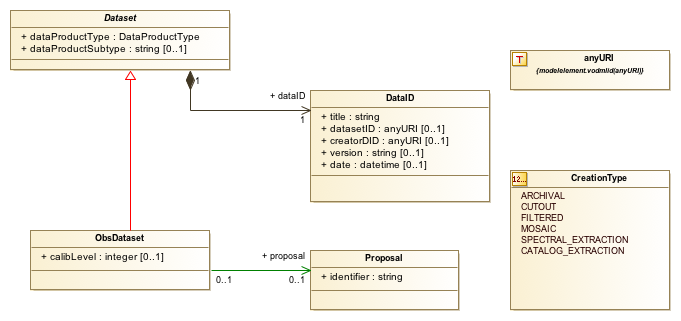
\includegraphics[width=0.9\textwidth]{diagrams/notation_example.png}}
    \caption{Notation example diagram}\label{fig:notation_example}
  \end{center}
  \end{figure}

  \subsubsection{ObjectType}
  \label{sect:ObjectType}
  ObjectTypes are represented by a plain box. The type name is annotated in the top window, abstract
types use italic typeface. Attributes, if any, are listed in the lower panel. Attributes may only be
of primitive type (real, string, etc), a defined DataType, or an Enumeration type. Relationships to
other objects are defined via the composition and reference relation arrows.

  \subsubsection{DataType}
  \label{sect:DataType}
  DataTypes are represented by a box shape similar to ObjectType, but annotated with a "T" symbol in the top left corner.

  \subsubsection{Enumerations}
  \label{sect:Enumerations}
  Enumerations are represented by a box shape similar to ObjectType, but annotated with a "1,2.."
symbol in the top left corner. Enumeration Literals (possible values) are listed below the
enumeration type name.

  \subsubsection{Generalization}
  \label{sect:Generalization}
  Generalizations are represented by a red line, with open triangle at the end of the source, or more general, object.

  \subsubsection{Composition}
  \label{sect:Composition}
  The composition relation is indicated by a black line with a solid diamond attached to the
containing object, and an arrow pointing to the object being contained. The composition relation is
very tight, where the container is responsible for the creation and existence of the target. Any
object may be in no more than one composition relation with any container. The attribute name
for the composition relation is annotated at the destination of the relation (e.g. "+ dataID"). This is
typically a lower-cased version of the destination type name, but this is not required.

  \subsubsection{Reference}
  \label{sect:Reference}
  The reference relation is indicated by a green line, with an arrow pointing to the object being
referenced. The reference relation is much looser than composition, the container has no
ownership of the target, but merely holds a pointer, or other indirect connection to it. The
attribute name is annotated at the destination of the relation ( e.g. "+ proposal"). This is typically
a lower-cased version of the destination type name, but may be another name indicating the role
that the element is playing in this context.

  \subsubsection{Multiplicity}
  \label{sect:Multiplicity}
  All attributes and relations have a multiplicity associated with them. For attributes, the multiplicity
is contained within brackets just after the attribute name. If no bracket is displayed, this is
equivalent to '[1]'.
\begin{itemize}
\item 1 = one and only one value must be provided.
\item 0..1 = zero or one value may be provided.
\item * = zero or more values may be provided (open ended).
\end{itemize}


\pagebreak
\subsection{Model Identification metadata}
\label{sect:stereotypes}

Interoperability of datasets requires that there be a standardized method for
identifying the specific type of dataset, and which model(s) and versions
thereof it conforms to. These elements are not properties of the dataset, but
rather, of the Model itself. We provide this information via stereotypes
assigned to the model packages (e.g. Dataset, Char, Meas, IVOA ).

  \subsubsection{Model stereotype}
  The Model stereotype (<<model>>) consists of a set of Model properties which
  identify a particular model and its dependencies. Each model should
  specifically state the appropriate values for these properties.

  \begin{itemize}
  \item \textbf{title:string[1]} \newline
    The model title or long name.
  \item \textbf{version:string[1]} \newline
    The version of this model. To be represented as a string with format "<version>.<subversion>"
  \item \textbf{name:string[1]} \newline
    Sometimes referred to as 'namespace’ or 'prefix', this is a tag which is
    used to label elements of a particular model. The value must match the name of
    the model package itself. This string identifies the particular model type 
    (eg. ds, char, meas). Each model must declare a prefix string which is
    unique within the IVOA to tag elements from those models. A typical use of the
    prefix is in the construction of element UTYPE strings.
  \item \textbf{url:anyURI[1]} \newline
    A URL from which the full model description may be obtained (e.g. XML schema).
  \item \textbf{imports:Import[*]} \newline
    Here, we specify which the models on which this model is dependent. This
    model uses and/or extends elements from the Characterisation and Measurements
    Data models. In this document, we provide descriptions and supporting
    information about usage of these objects in a particular context. The
    originating documents, however, remain the definitive source for element definitions.
  \end{itemize}

  \subsubsection{ImportStereotype}
  The <<modelimport>> stereotype is attached to Packages representing imported
  models. It identifies the model by name, and provides URLs from which the full
  description may be obtained.
  \begin{itemize}
  \item \textbf{name:string[1]} \newline
    The name of the imported model. This name MUST match the 'name' property of
    imported model's Model metadata.
  \item \textbf{version:string[1]} \newline
    The version of this model. To be represented as a string with format "<version>.<subversion>"
  \item \textbf{url:anyURI[1]} \newline
    A URL from which the full model description may be obtained (e.g. XML schema).
  \end{itemize}
  

\pagebreak
\subsection{Extensibility}
There is no formal mechanism in the IVOA defining how users may extend models
with their own content. However, the above Model identification metadata
provides a simple means to do so. Using this process, a user would model their
content as an extension of the IVOA standard.

  \subsubsection{Model}
    \begin{itemize}
    \item \textbf{name} \newline
      The user-defined model would need a name unique from that of the standard.
    \item \textbf{prefix} \newline
      A unique prefix must be defined for the user-defined model elements. Users
      must take care not to make use of prefix tags which are associated with
      current IVOA standards, (e.g. ’cha’, ’spec’, ’ssa’, ’meas’). At the time of
      this writing, there is no central repository of reserved namespace strings.
    \item \textbf{imports} \newline
      The user defined model should declare the IVOA standard being extended as
      an imported model. Fields for the imported model name and url may be obtained
      from that standard's documentation.
    \end{itemize}

  \subsubsection{Scope}
  We permit any object modeled in this document to be extended with user-
  defined content, with the following restrictions:
  \begin{itemize}
  \item Follow VO-DML modeling practices.
  \item Values of extended content must be consistent with the content of
        modeled data. That is, using the IVOA base primitive types, Quantity,
        and Coordinates as appropriate.
  \item Since extended content, by definition, does not follow the
        corresponding model, it is not possible for general applications to
        interpret complex structures within that content. It is, therefore,
        recommended that users define extended content in such a way as to
        avoid ambiguity between its components.
  \end{itemize}

  \subsubsection{Support}
  Applications should, but are not required to, provide the following support for extended content:
  \begin{itemize}
  \item Retain existence of extended content, including namespace and UTypes.
  \item Retain association with modeled component.
  \item Provide access to extended content by users.
  \end{itemize}
  
